\section*{Agradecimientos}

\vspace{0.5 cm}

El presente documento explica la implementación y funcionamiento del servicio de escritura de MQTT a base de datos relacional,
este proyecto fue realizado para el proyecto denominado \textit{Proyecto AV Geotel}, el cual tiene como objetivo
la creación de un sistema de monitoreo y control de una flota de vehículos, utilizando tecnologías de telemetría, IoT,
sistemas embebidos y bases de datos. Este componente del proyecto fue desarrollado por el alumno:

\begin{itemize}[noitemsep]
    \item Treviño Selles Jorge Eithan
\end{itemize}

\newpage

\section*{Acronimos}
\textbf{AV} - \textit{Autonomous Vehicle} - Vehículo Autónomo \\
\textbf{IoT} - \textit{Internet of Things} - Internet de las Cosas \\
\textbf{MQTT} - \textit{Message Queuing Telemetry Transport} - Protocolo de Mensajería para Telemetría \\
\textbf{DB} - \textit{Database} - Base de Datos \\
\textbf{SQL} - \textit{Structured Query Language} - Lenguaje de Consulta Estructurada \\
\textbf{PostgreSQL} - Sistema de Gestión de Bases de Datos Relacional \\
\textbf{Docker} - Plataforma de Contenerización utilizando contenedores \\
\textbf{Docker Compose} - Herramienta para definir y ejecutar aplicaciones Docker multi-contenedor \\
\textbf{Makefile} - Herramienta de automatización de tareas en proyectos de software \\
\textbf{PubSub} - \textit{Publish-Subscribe} - Modelo de Publicación-Suscripción \\
\textbf{IT} - \textit{Information Technology} - Tecnología de la Información \\
\textbf{CI/CD} - \textit{Continuous Integration/Continuous Deployment} - Integración Continua/Despliegue Continuo \\
\textbf{QA} - \textit{Quality Assurance} - Aseguramiento de la Calidad


\chapter{Objetivos}

\begin{itemize}[noitemsep]
    \item Documentar el proceso de implementación del servicio de escritura de MQTT a base de datos relacional.
    \item Explicar el funcionamiento del servicio de escritura de MQTT a base de datos relacional y su integración con el sistema de monitoreo y control de la flota de vehículos.
    \item Proporcionar una guía de uso y mantenimiento del servicio de escritura de MQTT a base de datos relacional.
    \item Facilitar la comprensión del despliegue del proyecto en un servidor remoto, utilizando Docker y Docker Compose.
    \item Proporcionar una guía de instalación y configuración del servicio de escritura de MQTT a base de datos relacional en un entorno local.
\end{itemize}

\chapter{Introducción}

En la era de la transformación digital y el Internet de las Cosas (IoT), la gestión inteligente de flotas vehiculares se ha convertido en una necesidad crítica para empresas de transporte, logística y servicios. La capacidad de monitorear en tiempo real parámetros como ubicación, velocidad, consumo de combustible, temperatura del motor y estado general de los vehículos no solo mejora la eficiencia operativa, sino que también contribuye significativamente a la seguridad vial y la reducción de costos operacionales.

\section{Contexto del Proyecto}

Las flotas vehiculares modernas generan grandes volúmenes de datos de telemetría que incluyen información crítica sobre el rendimiento del vehículo, patrones de conducción, rutas optimizadas y alertas de seguridad. Sin embargo, la gestión efectiva de estos datos requiere una arquitectura tecnológica que permita la recolección, procesamiento, almacenamiento y análisis de información en tiempo real
de forma eficiente, escalable y confiable.

Para abordar estas problemáticas, se desarrolló un \textbf{sistema integral de telemetría vehicular} basado en la arquitectura MQTT (Message Queuing Telemetry Transport) que permite la comunicación eficiente entre dispositivos IoT instalados en los vehículos y una base de datos relacional centralizada. MQTT es un protocolo ligero de mensajería diseñado para entornos con recursos limitados y redes inestables, ideal para aplicaciones IoT.
Se basa en un modelo de publicación-suscripción que facilita la escalabilidad y la eficiencia en la transmisión de datos.

\begin{figure}[h]
    \centering
    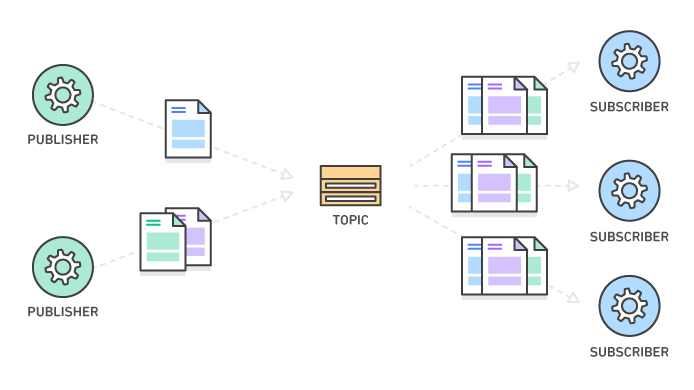
\includegraphics[width=0.8\textwidth]{Imagenes/2PubSub.png}
    \caption{Modelo de Publicación-Suscripción de MQTT. [1]}
    \label{fig:pubsub}
\end{figure}

El componente descrito en este documento es el \textbf{servicio de escritura de MQTT a base de datos relacional}, que actúa como intermediario entre los datos de telemetría generados por los vehículos y el sistema de almacenamiento persistente. Este servicio garantiza la integridad, disponibilidad y procesamiento en tiempo real de la información vehicular.

\subsection{Características Principales del Sistema}

\begin{itemize}[noitemsep]
    \item \textbf{Comunicación en tiempo real}: Utilización del protocolo MQTT para transmisión eficiente de datos de telemetría.
    \item \textbf{Almacenamiento robusto}: Base de datos PostgreSQL para garantizar la integridad y persistencia de los datos.
    \item \textbf{Arquitectura escalable}: Diseño basado en contenedores Docker para facilitar el despliegue y escalabilidad.
    \item \textbf{Monitoreo integral}: Capacidad de procesar múltiples parámetros vehiculares simultáneamente.
    \item \textbf{Alta disponibilidad}: Implementación de mecanismos de recuperación ante fallos y logging detallado.
\end{itemize}

\section{Arquitectura del Sistema}

El sistema implementado sigue una arquitectura de microservicios que separa claramente las responsabilidades y permite una mayor flexibilidad y mantenibilidad. Los componentes principales incluyen:

\begin{enumerate}[noitemsep]
    \item \textbf{Dispositivos IoT vehiculares}: Sensores y unidades de telemetría instaladas en los vehículos que recolectan datos en tiempo real.
    \item \textbf{Broker MQTT}: Servidor Mosquitto que gestiona la comunicación entre dispositivos y servicios.
    \item \textbf{Servicio de escritura}: Aplicación Python que procesa mensajes MQTT y los almacena en la base de datos.
    \item \textbf{Base de datos relacional}: PostgreSQL para almacenamiento persistente y consultas eficientes.
    \item \textbf{Interface de administración}: pgAdmin para gestión y monitoreo de la base de datos.
\end{enumerate}

\section{Justificación Tecnológica}

La selección de tecnologías para este proyecto se basó en criterios de rendimiento, escalabilidad, confiabilidad y facilidad de mantenimiento:

\subsection{Protocolo MQTT}
MQTT fue seleccionado como protocolo de comunicación debido a su eficiencia en entornos con limitaciones de ancho de banda, su modelo publish-subscribe que facilita la escalabilidad, y su amplia adopción en aplicaciones IoT.

\subsection{PostgreSQL}
La elección de PostgreSQL como sistema de gestión de base de datos se fundamenta en su robustez, capacidad de manejo de grandes volúmenes de datos, soporte para datos geoespaciales y su naturaleza open-source que reduce costos de licenciamiento.
Si bien existieron preocupaciones iniciales sobre la seguridad de Docker Desktop, utilizaremos exclusivamente Docker Engine dentro del servidor en el laboratorio, lo que garantiza un entorno seguro y controlado para el despliegue del sistema
basado en software libre.

\subsection{Python}
Python fue elegido como lenguaje de desarrollo principal por su extensa biblioteca de paquetes para IoT y bases de datos, su sintaxis clara que facilita el mantenimiento, y su excelente soporte para aplicaciones de procesamiento de datos en tiempo real.

\subsection{Docker y Docker Compose}
La containerización con Docker proporciona portabilidad, aislamiento de dependencias y facilita el despliegue en diferentes entornos, mientras que Docker Compose simplifica la orquestación de múltiples servicios.

\subsection{Makefile}
El uso de Makefile permite automatizar tareas comunes de desarrollo y despliegue, mejorando la eficiencia del flujo de trabajo y asegurando consistencia en las operaciones de construcción y ejecución del servicio

\section{Alcance del Documento}

Este documento técnico aborda de manera integral la implementación, configuración y mantenimiento del servicio de escritura de MQTT a base de datos relacional. Los lectores encontrarán:

\begin{itemize}[noitemsep]
    \item Análisis detallado de la arquitectura del sistema
    \item Guías paso a paso para la instalación y configuración
    \item Documentación completa de la estructura de datos y esquemas de base de datos
    \item Procedimientos de testing y validación del sistema
    \item Estrategias de monitoreo, diagnóstico y resolución de problemas
    \item Recomendaciones para despliegue en producción
    \item Consideraciones de seguridad y mejores prácticas
\end{itemize}

El documento está dirigido a desarrolladores, administradores de sistemas y en general personal técnico del laboratorio responsable de la implementación y mantenimiento del sistema de telemetría vehicular y/o
infraestructura de IT. Se espera que sirva como una guía completa para la comprensión y operación del servicio de escritura de MQTT a base de datos relacional, facilitando su integración en el ecosistema de monitoreo y control de flotas vehiculares.
